\Introduction

В природе гранулярная материя является одним из самых распространенных типов вещества, начиная от песка под нашими ногами,
сахара для чая, различных порошков для строительства и техногенного производства, заканчивая космической пылью в аккреционных дисках 
зарождающихся звездных и галактических системах. Гранулярная материя характеризуется в основном диссипативными свойствами при контактном
взаимодействии составных частиц. Частный случай гранулярных систем, так называемый \emph{гранулярный газ}, является объектом интереса
в нашей работе \cite{Brilliantov:2004book}. Под газообразной мы будем подразумевать систему в которой все контактные взаимодействия бинарные, 
т.е. в любой момент времени во всех взаимодействиях участвуют только два объекта, а тройные, четверные и т.д. взаимодействия исключены.
Таким образом, подобная система может быть описана классическими уравнениями Больцмана-Энскога.

Объектом наших исследований являются кольца Сатурна. 
Данный выбор был неслучаен, и был стимулирован успехом масштабного проекта NASA, Европейского Космического Агентства и Итальянского
Космического Агентства -- миссия Кассини-Гюйгенс. В рамках этого проекта, 15 октября 1997 года, на орбиту вокруг Сатурна был отправлен космический
исследовательский аппарат Кассини. Целью данной миссии было исследование планеты Сатурн, его колец и лун. На борту космического аппарата находилась
автоматическая станция Гюйгенс, предназначенная для посадки на Титан, крупнейший из лун Сатурна. 1 июля 2004 года, комплекс вышел на орбиту вокруг Сатурна.
25 декабря 2004 года, станция Гюйгенс отделилась от основного комплекса и 14 января 2005 года вошла в атмосферу Титана. Изначально миссия была 
запланирована до 2008 года, однако была несколько раз продлена, и в итоге 15 сентября 2017 года космический аппарат Кассини завершил свою миссию,
пролетев в непосредственной близости от колец и вошел в атмосферу Сатурна. 
Пример снимка сделанного аппаратом Кассини в 2009 году показан на Рис.~\ref{fig:cassini_saturn_panorama}.
Весь масштаб данной миссии можно привести в виде статистических данных 
(Табл.~\ref{tab:cassini_mission}). 
\begin{table}[ht]    
    \caption{Итоговая статистика миссии Кассини-Гюйгенс по окончании 20 летнего периода активности}
    \begin{tabular}{|l|l|}
    \hline    
        Общая стоимость проекта             & около 3,26 миллиард долларов США  \\
        Длительность миссии                 & 19 лет, 335 дней                  \\
        Объем полученных научных данных     & 635 Гб                            \\
        Найдено новых лун                   & 6 наименованных                   \\
        Количество стран участниц           & 27 стран со всего мира            \\
        Опубликовано научных публикаций     & 3 948                             \\
        Сделано снимков                     & 453 048                           \\
    \hline    
    \end{tabular}
    \label{tab:cassini_mission}
\end{table}

\begin{figure}[ht]
    \centering
    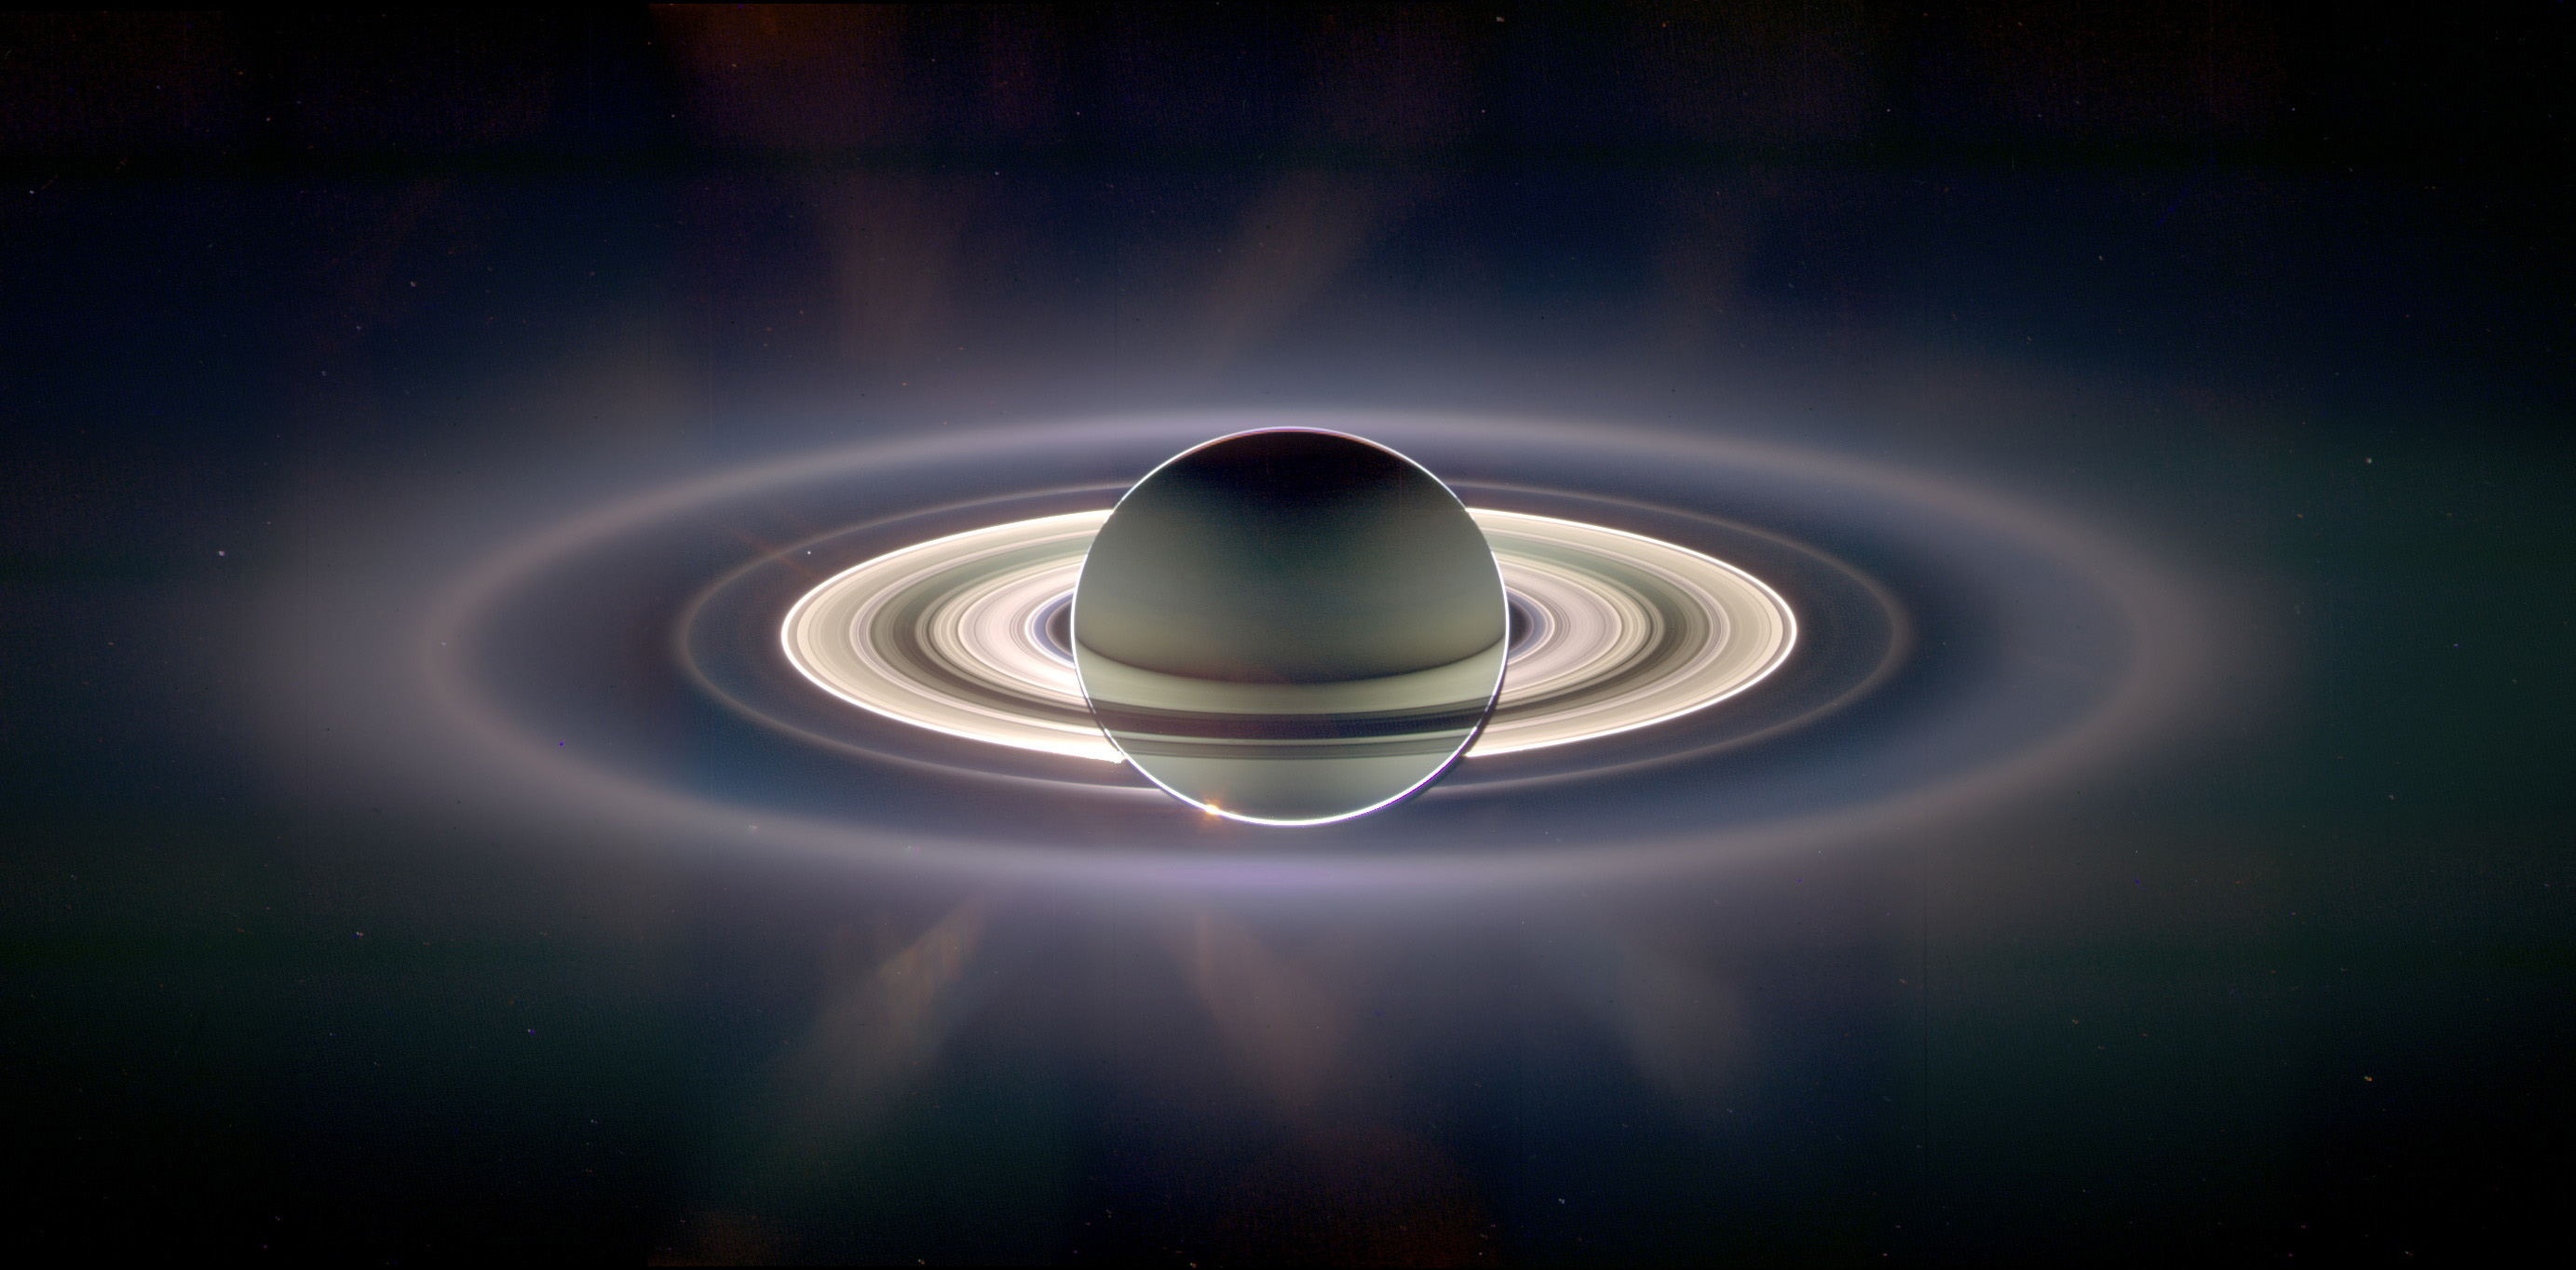
\includegraphics[width=\textwidth]{figures/newrings_cassini_big.jpg}
    \caption{Фотография Сатурна и его колец отправленная аппаратом Кассини в октябре 2009 года}
    \label{fig:cassini_saturn_panorama}
\end{figure}

Большая доля этих исследований посвящено изучению динамики и свойств колец Сатурна, которые являются ярким примером гранулярных газов в природе. 
Сами кольца состоят в основном из водяного льда и силикатных образований. Размеры частиц материала кольца составляют от микрометров до нескольких 
десятков метров. Объекты б\'{о}льших размеров, от нескольких сот метров до километров и более, классифицируются уже как отдельные луны Сатурна. 
Некоторые из подобных лун, как Пан и Дафнис (которые были обнаружены аппаратом Кассини), вращаются вокруг Сатурна на орбитах, находящихся внутри самих колец, 
имеют свое гравитационное поле которое серьезно воздействует на динамику мелких объектов кольца. Однако в нашей работе мы ограничимся системами, 
размеры составляющих частиц которых не превышают порядка нескольких метров. 
В этом случае можно исключить из рассмотрения гравитационные взаимодействия и сконцентрироваться только на контактных, механических
взаимодействиях при описании динамики гранулярного газа.

Для простоты описания механики столкновения частиц газа, будем рассматривать их как сферические объекты с заданными параметрами как
масса $m$, радиус $r$, модуль Юнга $Y$, коэффициент Пуассона $\eta$, поверхностная энергия (адгезивность) $\gamma$, коэффициент вязкой диссипации $A$.
Обозначенные выше параметры будут использованы для построения компьютерной модели столкновений, однако для теоретического описания системы
все механические свойства объединены в единый параметр, так называемый \emph{коэффициент реституции} -- $\eps$. Для описания динамики сухих
гранулярных газов, коэффициент реституции играет ключевую роль, и показывает количество диссипированной энергии при столкновениях. Математически
описывается следующим образом:
\begin{equation}\label{eq:restitution}
    \bg'_{12} = -\eps\bg_{12}\;,
\end{equation}
где $\bg_{12}$ -- относительная скорость частиц $1$ и $2$ \emph{до} столкновения, $\bg'_{12}$ -- относительная скорость \emph{после} столкновения.
Коэффициент реституции в общем случае всегда лежит в пределах $0\leq\eps\leq 1$. При $\eps = 0$ -- мы имеем абсолютно неупругое столкновение, 
при $\eps = 1$ -- абсолютно упругое столкновение. В данной работе мы будем рассматривать только сухие гранулярные системы, т. е. такие
системы для которых коэффициент адгезивности $\gamma = 0$. Таким образом, контактные взаимодействия частиц можно полностью описать двумя параметрами:
$r$ -- линейный размер частицы, который характеризует массу ($m\propto r^3$), поверхностное сечение ($\sigma\propto r^2$) и т.д., 
и $\eps$ -- коэффициент реституции, который описывает диссипативные свойства материала частицы. Мы будем предполагать, что материал частиц 
везде единообразен, и для всех столкновений $\eps$ будет одинаковый. 

Основным свойством гранулярного газа является его диссипативность, и как результат его \emph{гранулярная температура} имеет свойство всегда уменьшаться, 
т.е. предоставленный самому себе гранулярный газ, всегда будет \emph{охлаждаться}. Данное явление носит название закона Хаффа:
\begin{equation}
    T(t) = \frac{T_0}{(1+t/\tau_0)^2}\;, 
\end{equation}
где
\begin{equation}
    \tau^{-1}_0\propto n\sigma^2\left(1-\eps^2\right)\sqrt{T_0}\;.
\end{equation}
Таким образом, если в систему не подводить внешний источник энергии, то со временем гранулярный газ придет к состоянию с нулевой энергией. Здесь мы
коротко упомянули понятие гранулярной температуры, по аналогии с температурой обычных систем, однако оно не является температурой материала частицы 
в обычном понимании. Более детально мы рассмотрим ее в основной части работы.

Следующим важным моментом является \emph{полидисперсность} системы. До этого мы считали что все частицы в газе одинакового размера, однако в реальных
системах планетарных колец, размеры частиц очень сильно варьируются. Данное свойство привносит в систему один существенный эффект: если рассматривать
полидисперсную систему как смешение большого количества монодисперсных гранулярных газов с различными размерами, то парциальная температура каждого
из этих газов становится отличной друг от друга. Чем больше разница между размерами частиц этих монодисперсных газов, тем больше их разница в
гранулярной температуре. Конечно, без внешнего источника энергии, все эти температуры со временем сравняются и станут нулевыми. Однако планетарные
кольца находятся в центральном гравитационном поле своей планеты, и на самом деле являются дисками с дифференциальным вращением, и гранулярная система
подпитывается за счет гравитационной энергии своей планеты. Более подробно мы остановимся на данном явлении в основной части работы. Здесь же,
укажем что за счет данной подкачки энергии, температуры всех отдельных частей системы остановятся на определенном и различном стационарном значении, 
что является одним из результатов нашей работы. А также, мы покажем что подобная разница в стационарных температурах системы, оказывает влияние
на радиальное распределение размеров частиц друг относительно друга. Данный эффект неодинакового распределения частиц по размерам относительно
центрального поля хорошо виден на Рис.~\ref{fig:cassini_rings_radial_sizes}.

\begin{figure}[ht]
    \centering
    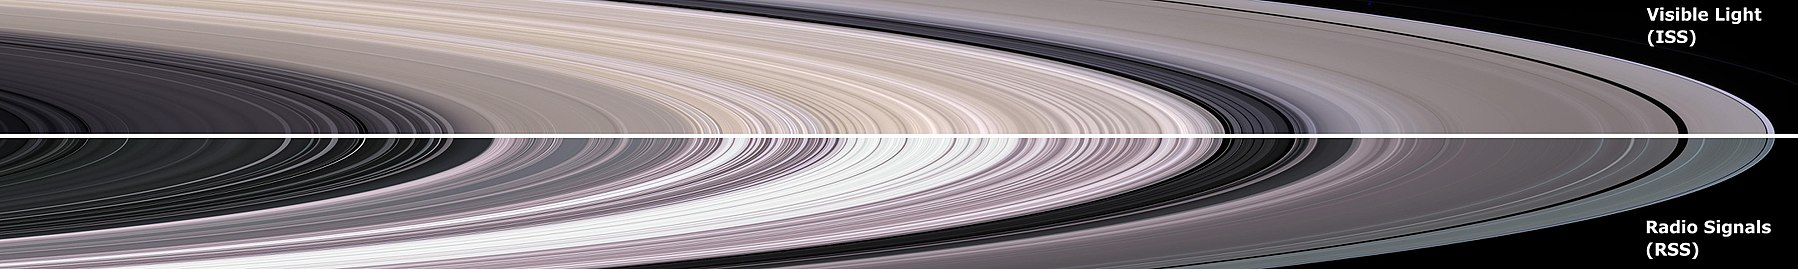
\includegraphics[width=\textwidth]{figures/1800px-Saturn's_rings_in_visible_light_and_radio.jpg}
    \caption{Фотография колец Сатурна в радиальном срезе. Верхняя часть показана в оптическом диапазоне, нижняя в радиоволновом диапазоне, 
    где цвета соотнесены с размерами частиц}
    \label{fig:cassini_rings_radial_sizes}
\end{figure}